% Informe final SI3003 - Agente de calidad del aire del Valle de Aburrá
% Compilar desde docs/:  pdflatex informe.tex  (dos veces para referencias)
\documentclass[10pt,a4paper]{article}

\usepackage[utf8]{inputenc}
\usepackage[T1]{fontenc}
\usepackage[spanish,es-noshorthands,es-tabla]{babel}
\usepackage{lmodern}
\usepackage{textcomp}
\usepackage[margin=2cm]{geometry}
\usepackage{amsmath,amssymb}
\usepackage{booktabs}
\usepackage{tabularx}
\usepackage{graphicx}
\usepackage{enumitem}
\usepackage{xcolor}
\usepackage[hidelinks]{hyperref}
\usepackage{caption}

\setlist{nosep,leftmargin=1.2em}
\setlength{\parskip}{3pt}
\setlength{\parindent}{0pt}
\setlength{\emergencystretch}{1.5em}
\captionsetup{font=small,labelfont=bf}
\graphicspath{{../results/figures/}}

\newcommand{\ugm}{\,\textmu g/m\textsuperscript{3}}
\newcommand{\code}[1]{\texttt{\small #1}}
\newcommand{\pmd}{PM\textsubscript{2.5}}

\title{\vspace{-1.2cm}\textbf{Agente de calidad del aire del Valle de Aburrá}\\[2pt]
\large Naive Bayes y HMM propios + agente LLM con RAG + dashboard}
\author{SI3003 -- Inteligencia Artificial, EAFIT 2026-1 $\cdot$ Proyecto final (idea 3.1)\\
Grupo: \textit{[completar]}}
\date{Noviembre de 2026}

\begin{document}
\maketitle
\vspace{-0.6cm}

\section{Problema}
El Valle de Aburrá vive episodios de contaminación por \pmd, sobre todo entre febrero y abril y, en
menor medida, en octubre y noviembre. Para un ciudadano no es obvio qué significa un valor en \ugm,
qué tan probable es que mañana empeore ni qué recomienda la norma. Construimos un MVP que combina tres
piezas: (i) modelos clásicos propios que estiman la categoría del día siguiente; (ii) un agente LLM
con \textit{tool calling} y RAG que responde en lenguaje natural citando normativa; y (iii) un
dashboard que integra mapa, serie de tiempo, predicción y chat.

\section{Datos}
\begin{itemize}
  \item \textbf{Fuente principal:} IDEAM-SISAIRE (datos.gov.co, conjunto \code{g4t8-zkc3}), con \pmd{}
    horario medido por las estaciones del AMVA entre 2020 y 2025 (1\,046\,932 filas). El portal del AMVA
    respondió 502 y SIATA solo publica una ventana de un año (jul-2023 a jul-2024), que usamos para
    rellenar 46\,117 horas.
  \item \textbf{Meteorología:} lluvia y viento diarios de Open-Meteo (reanálisis ERA5, \textit{modelado}),
    en 8 celdas de 0,1\textdegree.
  \item \textbf{Limpieza:} promedio de 24\,h solo con $\geq$\,75\,\% de horas válidas (1\,922 días-estación
    descartados). Encontramos una \textbf{inconsistencia de escala} en SISAIRE: varias estaciones reportan
    en 2020--2023 medianas de 60 a 117\ugm, frente a $\sim$15 en las vecinas. Si no se filtra, aparecen
    cientos de días ``críticos'' falsos. Descartamos 715 estación-mes con dos reglas: mediana mensual
    mayor a 3 veces el P25 regional del mes, o mayor a 3 veces la mediana propia de la estación en 2024--2025.
  \item \textbf{Resultado:} 25 estaciones y 28\,304 días-estación.
  \item \textbf{Clases del proyecto:} \code{normal} ($\leq 37$\ugm, el límite diario de la Res.~2254/2017
    desde jul-2018), \code{alerta} (38--55) y \code{critico} ($\geq 56$). Por rangos, coinciden con los
    niveles de Prevención y de Alerta/Emergencia de la Tabla~4 de la resolución, pero son una
    simplificación nuestra, no una declaratoria.
  \item \textbf{Desbalance extremo:} 27\,996 días normal, 307 alerta y \textbf{1} crítico. Las alertas se
    concentran en feb--abr (EDA en \code{notebooks/01\_eda.ipynb}).
\end{itemize}

\section{Parte 1: modelos clásicos (implementación propia en NumPy)}
\textbf{Naive Bayes categórico} (\code{src/models/naive\_bayes.py}). Predice la clase de $t+1$ a partir
de features del día $t$:
\begin{itemize}
  \item nivel de \pmd{} (5 rangos);
  \item tendencia frente a $t-1$;
  \item terciles de lluvia y viento, calculados solo con entrenamiento;
  \item mes y día de la semana de $t+1$ (calendario conocido de antemano).
\end{itemize}
Con suavizado de Laplace y en log-probabilidades:
\begin{equation*}
  \log P(y{=}k \mid \mathbf{x}) = \log P(y{=}k) + \sum_j \log \frac{N_{k,j,x_j} + \alpha}{N_k + \alpha V_j} - \log Z .
\end{equation*}
El prior empírico se suaviza (\code{prior\_alpha = 1}) porque en entrenamiento no hay ningún día
crítico. Un test verifica que \code{predict\_proba} coincide con \code{sklearn.CategoricalNB}
(tolerancia $10^{-6}$).

\textbf{HMM gaussiano de 3 estados} sobre $x_t = \log(\text{\pmd})$ (\code{src/models/hmm.py}):
\begin{itemize}
  \item forward escalado, backward, Baum-Welch sobre las 25 series y Viterbi;
  \item los días faltantes se tratan como observaciones ausentes ($b_s(x_t)=1$);
  \item la predicción a un paso es $P(z_{t+1}\mid x_{1:t}) = A^{\top}\alpha_t$, y se convierte en
    probabilidad de clase integrando la gaussiana de cada estado sobre los rangos de \pmd.
\end{itemize}
Los tests comprueban que la log-verosimilitud sea monótona y que se recuperen los parámetros en datos simulados.

\textbf{Protocolo.} Partición temporal por fecha objetivo: entrenamiento 2020--2023 y prueba 2024--2025.
La prueba abarca dos años porque 2025 solo tiene 6 días de alerta, mientras que 2024 incluye el
episodio de marzo. Los hiperparámetros del NB ($\alpha \in \{0{,}5;\,1;\,2;\,5\}$, prior empírico/uniforme
y umbral de decisión) se eligieron con validación de ventana expandible en 2021, 2022 y 2023. Resultado:
$\alpha = 5$, prior empírico, argmax. Líneas base: persistencia y climatología mensual.

\begin{table}[h]
\centering\small
\caption{Prueba 2024--2025 ($n = 14\,744$). Episodio = alerta o crítico. El F1 macro incluye las 3
clases; ``crítico'' tiene un solo caso en prueba.}
\begin{tabular}{lccccc}
\toprule
Modelo & Accuracy & F1 macro & Recall episodios & Precisión episodios & Log-loss \\
\midrule
Persistencia          & 0,987 & \textbf{0,511} & \textbf{0,549} & 0,543 & --- \\
Climatología mensual  & 0,986 & 0,331 & 0,000 & --- & 0,065 \\
\textbf{Naive Bayes}  & \textbf{0,989} & 0,505 & 0,451 & \textbf{0,628} & \textbf{0,039} \\
HMM (1 paso)          & 0,986 & 0,331 & 0,000 & --- & 0,058 \\
\bottomrule
\end{tabular}
\end{table}

\begin{figure}[h]
\centering
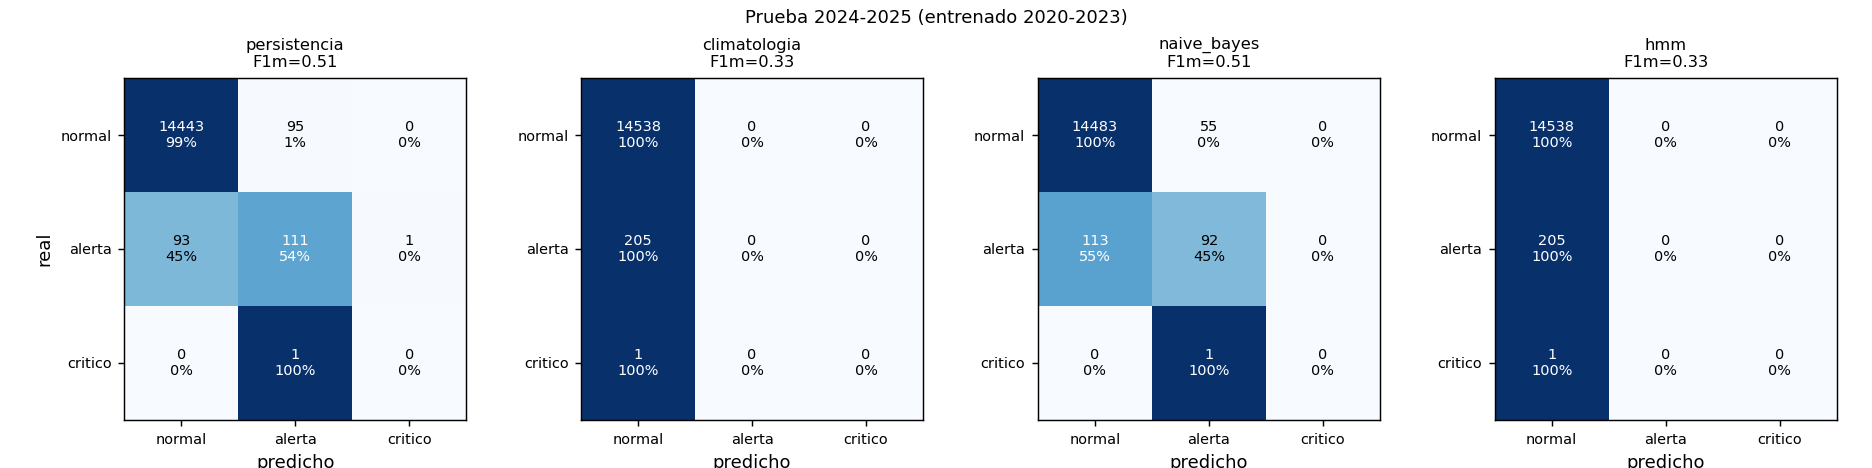
\includegraphics[width=\linewidth]{confusion_test.png}
\caption{Matrices de confusión en prueba (normalizadas por fila).}
\end{figure}

\textbf{Interpretación.}
\begin{itemize}
  \item \textbf{El NB no supera a la persistencia en F1 macro; empatan.} El NB acierta más cuando anuncia
    un episodio (precisión 0,63 vs 0,54) pero detecta menos (recall 0,45 vs 0,55). Su aporte real son
    probabilidades útiles: log-loss 0,039 frente a 0,065 de la climatología.
  \item \textbf{Por qué no gana:} el \pmd{} es muy persistente ($\rho = 0{,}74$ entre días consecutivos), y
    la meteorología disponible es del día $t$, de baja resolución y poco correlacionada con el \pmd{} de
    mañana ($|\rho| < 0{,}1$).
  \item \textbf{Ajuste descartado:} discretizar el nivel de hoy más fino cerca de 37\ugm{} no mejoró la
    validación, así que no se adoptó (no ajustamos sobre prueba).
  \item \textbf{HMM:} sus estados quedaron en niveles de fondo ($\sim$12, 17 y 25\ugm), no en episodios,
    porque el entrenamiento casi no tiene alertas (74 de 12\,662). Como clasificador equivale a la
    climatología, aunque con mejor log-loss. En el dashboard lo usamos como descriptor del estado latente.
\end{itemize}

\section{Parte 2: agente LLM con RAG}
\textbf{Loop} (\code{src/agent/loop.py}), escrito sin frameworks:
\begin{enumerate}
  \item Arma los mensajes: \textit{system prompt}, contexto del dashboard (estación y fecha), historial y pregunta.
  \item Llama al LLM con 4 herramientas en JSON Schema y ejecuta las que pida.
  \item Devuelve el resultado como mensajes \code{tool} y repite hasta la respuesta final o
    $T_{\max} = 6$; en la última iteración quita las herramientas para forzar una respuesta.
\end{enumerate}
Los errores de herramientas vuelven como \code{\{"error": ...\}} y el LLM tiene un reintento único que
respeta \code{retry-after} ante un 429. Cada paso queda en una traza (herramienta, argumentos, resumen,
latencia) que el dashboard muestra.

\textbf{Herramientas:} \code{get\_pm25} (dato diario, ICA y últimos 7 días); \code{predict\_tomorrow}
(NB y HMM, con features usadas y desempeño en prueba); \code{search\_docs} (RAG); \code{list\_stations}.

\textbf{RAG} (\code{src/rag/}). Corpus de 7 PDF: Res.~2254/2017, Acuerdo Metropolitano 15 (POECA),
resolución de episodio 2022, hoja metodológica ICA del IDEAM, resumen de las guías OMS 2021,
presentación OPS y plan POECA de La Estrella. Los fragmentos tienen $\sim$350 palabras con 60 de
solapamiento, siempre dentro de una página, para que la cita \code{[fuente, p. N]} sea exacta. Usa
\code{paraphrase-multilingual-MiniLM-L12-v2} con FAISS (coseno, umbral 0,40) y BM25 como respaldo sin internet.

\textbf{Hallazgos en las primeras pruebas y correcciones:}
\begin{itemize}
  \item el modelo agregó recomendaciones sin respaldo (mascarilla N95, hidratación) $\rightarrow$ el
    prompt exige que cada recomendación salga de un fragmento, con su cita al lado;
  \item atribuyó un texto de La Estrella al Acuerdo 15 $\rightarrow$ cada fragmento trae un campo
    \code{cita} para copiar literal, y el loop \textbf{verifica} que toda cita de la respuesta corresponda
    a un fragmento recuperado.
\end{itemize}

\section{Evaluación del agente}
\code{eval/questions.yaml} tiene 14 preguntas fijas: dato puntual (2), predicción (2, una con el
contexto del dashboard), normativa (2), salud (2), cadenas de 2 y 3 herramientas, estación inexistente,
fecha sin datos, pregunta fuera de alcance y una solicitud de consejo médico. \code{python eval/run\_eval.py}
las corre todas y califica cada una \textbf{automáticamente}. Una respuesta es correcta si se cumplen
todas estas condiciones: usó las herramientas esperadas; contiene los datos mínimos verificados de
antemano; tiene citas, si se requieren, y todas corresponden a fragmentos realmente recuperados; y no
hubo error del LLM.

\begin{table}[h]
\centering\small
\caption{Resultados de la evaluación (\code{openai/gpt-oss-120b} en Groq).}
\begin{tabular}{lccc}
\toprule
Corrida & Correctas & Herramientas esperadas & Citas correctas \\
\midrule
1                          & 12/14 (86\,\%) & 14/14 & 6/6 \\
2, tras corregir el prompt & \textbf{13/14 (93\,\%)} & 14/14 & 6/6 \\
\bottomrule
\end{tabular}
\end{table}

\textbf{Análisis de fallos (corrida 1).}
\begin{itemize}
  \item \textit{Dato puntual sin valor} (prompt): dio la categoría pero no los \ugm{} $\rightarrow$ regla
    ``incluye siempre el valor, la fecha y la categoría''.
  \item \textit{Niveles de declaratoria} (corpus + prompt): usó la tabla del Acuerdo 15, que adopta los
    cortes de la EPA de 2012, e inventó una fila de ``prevención'' $\rightarrow$ reglas de no completar
    tablas y de priorizar la norma nacional cuando las fuentes difieren.
\end{itemize}
En la corrida 2 ya no inventa la fila y declara que no tiene respaldo para ``prevención'', pero sigue
sin dar 38/56/151. El fragmento correcto (Res.~2254, p.~5) \textbf{sí se recupera}: el problema es el
OCR de esa tabla (\code{PM2.s'* 24 horas 38-55 56-150 2::151}). Queda como fallo reportado. La solución
sería reemplazar la copia escaneada por el texto oficial en HTML; no ajustamos la pregunta para que pase.
Latencia mediana $\approx$ 11\,s; los picos de hasta $\sim$100\,s se deben a las esperas por el límite de
tokens por minuto del plan gratuito.

\section{Dashboard}
\code{app.py} (Streamlit + Plotly) muestra:
\begin{itemize}
  \item mapa de estaciones coloreado por la categoría ICA del día elegido;
  \item serie de tiempo con bandas ICA, la línea de 37\ugm{} y una franja con el estado latente filtrado del HMM;
  \item tarjeta de predicción con barras de probabilidad (NB y HMM) y desempeño en prueba;
  \item chat que recibe la estación y fecha seleccionadas, con un expander ``¿Cómo llegó a esta
    respuesta?'' que muestra herramientas, citas y citas no verificadas.
\end{itemize}
Arranca sin internet y sin API key (chat desactivado con aviso), y lo prueban
\code{tests/test\_app.py} con \code{AppTest}.

\section{Limitaciones}
\begin{itemize}
  \item Solo hay un día crítico en seis años y $\sim$1\,\% de días de alerta: las métricas de episodios
    dependen sobre todo del episodio de feb--abr de 2024.
  \item En 2020--2023 falta la mitad de las estaciones por la inconsistencia de SISAIRE, y 2020 incluye
    la cuarentena por COVID-19.
  \item La meteorología es reanálisis de $\sim$10\,km y del día $t$; un pronóstico meteorológico de
    $t+1$ mejoraría la predicción.
  \item El POECA del corpus es el Acuerdo 15 (versión SICLAS), no el Acuerdo 04 de 2018 vigente, que no
    pudimos descargar. La Res.~2254 viene de una copia con OCR.
  \item La evaluación del agente es automática, con criterios por palabras clave: no mide la calidad de
    la redacción y puede castigar respuestas correctas formuladas de otra manera.
  \item El plan gratuito de Groq limita los tokens por minuto; la app maneja el 429, pero hay que
    espaciar las preguntas.
\end{itemize}

\vspace{4pt}
{\small\textit{Herramienta académica: no es consejo médico ni aviso oficial.}\\
\textit{Uso de IA generativa declarado en} \code{docs/declaracion\_ia.md}.}

\end{document}
